

\section{Le modèle de régression linéaire multiple}
\label{sec:ModèleEtNotation}

Le modèle de régression linéaire multiple constitue une généralisation du modèle de régression linéaire simple permettant d'étudier la relation une variable réponse $Y$ avec $p$ variables explicatives  $x_1, x_2, ..., x_p$. L'équation du modèle de régression linéaire multiple s'exprime de la manière suivante
\begin{align}\label{eq:reg_lin_mult}
	Y_i = \beta_0 + \beta_1 x_{i1} +  \beta_2 x_{i2}+ \ldots + \beta_p x_{ip} + \varepsilon_i, \;\;\;\;\;\; i=1,\ldots,n;\;\;\; j=1,\ldots,p,
\end{align}
où
\begin{itemize}
\item $Y_i$ est une variable aléatoire représentant la réponse de l'unité $i$;
\item $x_{ij}$ est la valeur (connue) de la $j$-ème variable explicative de l'unité $i$;
\item $\beta_0$ et $\beta_j,\, j=1,\dots, p$, sont les paramètres du modèle;
\item $\varepsilon_i$ est une variable aléatoire représentant le terme d'erreur de l'unité $i$.
\end{itemize}
Notons 
\begin{itemize}
\item $n$, le nombre d'observations;
\item $p$, le nombre de variables explicatives;
\item $p'=p+1$, le nombre de paramètres à estimer;
\item $\boY = \begin{pmatrix} Y_1 & \cdots & Y_n \end{pmatrix}^\top$, le vecteur $n \times 1$ contenant les $n$ observations à venir (pas encore observées) de la variable réponse;
\item $\bobeta = \begin{pmatrix} \beta_0 & \beta_1 & \cdots & \beta_p \end{pmatrix}^\top$, le vecteur $p' \times 1$ contenant les $p'$ coefficients de régression;
\item $\boeps = \begin{pmatrix} \varepsilon_1 & \cdots & \varepsilon_n \end{pmatrix}^\top$, le vecteur $n\times 1$ des termes d'erreur;
\item $\boX$, la matrice de design (ou d'incidence) $n \times p'$ contenant les observations des $p$ variables explicatives (incluant une colonne de 1 associée à $\beta_0$),
$$\boX = \begin{pmatrix}
        1 & x_{11} & x_{12} & \cdots & x_{1p}  \\
        1 & x_{21} & x_{22} & \cdots & x_{2p}  \\
        \vdots & \vdots & \vdots & \ddots & \vdots \\
        1 & x_{n1} & x_{n2} & \cdots & x_{np}  
    \end{pmatrix}.$$
\end{itemize}
Le modèle de régression linéaire multiple peut s'écrire à l'aide d'une notation matricielle,
\begin{align}
    \underbrace{\begin{pmatrix}
        Y_1 \\
        Y_2  \\
        \vdots \\
        Y_n
    \end{pmatrix}}_{n\times 1}
    &=
    \underbrace{\begin{pmatrix}
        1 & x_{11} & x_{12} & \cdots & x_{1p}  \\
        1 & x_{21} & x_{22} & \cdots & x_{2p}  \\
        \vdots & \vdots & \vdots & \ddots & \vdots \\
        1 & x_{n1} & x_{n2} & \cdots & x_{np}  
    \end{pmatrix}}_{n \times (p+1)}
    \underbrace{\begin{pmatrix}
        \beta_0 \\
        \beta_1 \\
        \vdots \\
        \beta_p 
    \end{pmatrix}}_{(p+1) \times 1}
    +
    \underbrace{\begin{pmatrix}
        \varepsilon_1 \\
        \varepsilon_2 \\
        \vdots \\
        \varepsilon_n 
    \end{pmatrix}}_{n \times 1}, \nonumber
    \intertext{que l'on écrit}
    \boY &= \boX \bobeta + \boeps.
    \label{eq:reg_lin_mult_mat}
\end{align}


\begin{exemple}\label{RLSRLM1}
Dans le cas de la régression linéaire simple, $p=1$ et on peut écrire
\begin{align*}
    \boY = \underbrace{\begin{pmatrix}
        Y_1 \\
        Y_2  \\
        \vdots \\
        Y_n
    \end{pmatrix}}_{n\times 1}, \quad
    \boX =
    \underbrace{\begin{pmatrix}
        1 & x_{1}   \\
        1 & x_{2}  \\
        \vdots & \vdots \\
        1 & x_{n}  
    \end{pmatrix}}_{n \times 2}, \quad
    \bobeta = \underbrace{\begin{pmatrix}
        \beta_0 \\
        \beta_1 
    \end{pmatrix}}_{2 \times 1}, \quad
    \boeps = \underbrace{\begin{pmatrix}
        \varepsilon_1 \\
        \varepsilon_2 \\
        \vdots \\
        \varepsilon_n 
    \end{pmatrix}}_{n \times 1}, 
\end{align*}
On a alors
\begin{align*}
    \begin{pmatrix}
        Y_1 \\
        Y_2  \\
        \vdots \\
        Y_n
    \end{pmatrix}
    =
    \begin{pmatrix}
        1 & x_{1}   \\
        1 & x_{2}  \\
        \vdots & \vdots \\
        1 & x_{n}  
    \end{pmatrix}
    \begin{pmatrix}
        \beta_0 \\
        \beta_1 
    \end{pmatrix}
    +
    \begin{pmatrix}
        \varepsilon_1 \\
        \varepsilon_2 \\
        \vdots \\
        \varepsilon_n 
    \end{pmatrix}
    =
    \begin{pmatrix}
        \beta_0 + \beta_1 x_1 + \varepsilon_1 \\
        \beta_0 + \beta_1 x_2 + \varepsilon_2 \\
        \vdots \\
        \beta_0 + \beta_1 x_n + \varepsilon_n
    \end{pmatrix}, 
\end{align*}
et le modèle de régression linéaire simple défini à l'équation \eqref{eq:reg_lin_simple} peut s'exprimer 
\begin{equation*}
\boY=\boX\bobeta+\boeps.
\end{equation*}
\end{exemple}

\subsection{Postulats du modèle de RLM}
\label{sec:PostulatsRLM}

Les postulats émis sur le modèle de régression linéaire multiple sont les mêmes que ceux émis sur le modèle de régression linéaire simple. Pour $i, \, j=1, \dots, n$, on a
\begin{enumerate}
  \item[$\mathcal{P}_1$.] La linéarité de la relation entre la variable réponse et les variables explicatives, $\esp[\varepsilon_i]=0$;
 \item[$\mathcal{P}_2$.] L'homoscédasticité (variance constante) des observations de la variable réponse, $\var[\varepsilon_i]=\sigma^2$;
 \item[$\mathcal{P}_3$.] L'indépendance des observations de la variable réponse, $\cov(\varepsilon_i,\varepsilon_j)=0 \mbox{ pour } i \neq j$;
 \item[$\mathcal{P}_4$.] La normalité des termes d'erreur, $\varepsilon_i \sim \N(0,\sigma^2)$.
\end{enumerate}


\subsection{Interprétation des paramètres}
\label{sec:InterpétationRLM}

Dans le modèle de RLM  défini à l'équation~\eqref{eq:reg_lin_mult}, et sous le postulat $\mathcal{P}_1. \; \esp[\varepsilon_i]=0$ pour $i=1, \dots, n$, le coefficient $\beta_0$ représente la valeur moyenne de $Y_i$ lorsque $x_{i1}, \ldots, x_{ip}$ prennent toutes simultanément la valeur 0. Le coefficient $\beta_j$, $j=1, \dots, p$, représente la variation dans la moyenne de $Y_i$ lorsque $x_j$ augmente d'une unité et que la valeur de toutes les autres variables explicatives reste constante.

Dans le modèle de régression linéaire simple, les points $Y$ sont situés autour d'une droite, alors que dans le modèle de régression linéaire multiple, ils sont dispersés autour d'un hyperplan.  Le coefficient $\beta_j$ représente la pente de l'hyperplan dans la direction de la variable explicative $j$. Voir la figure \ref{fig:rlm}.
\begin{figure}[h!]
\centerline{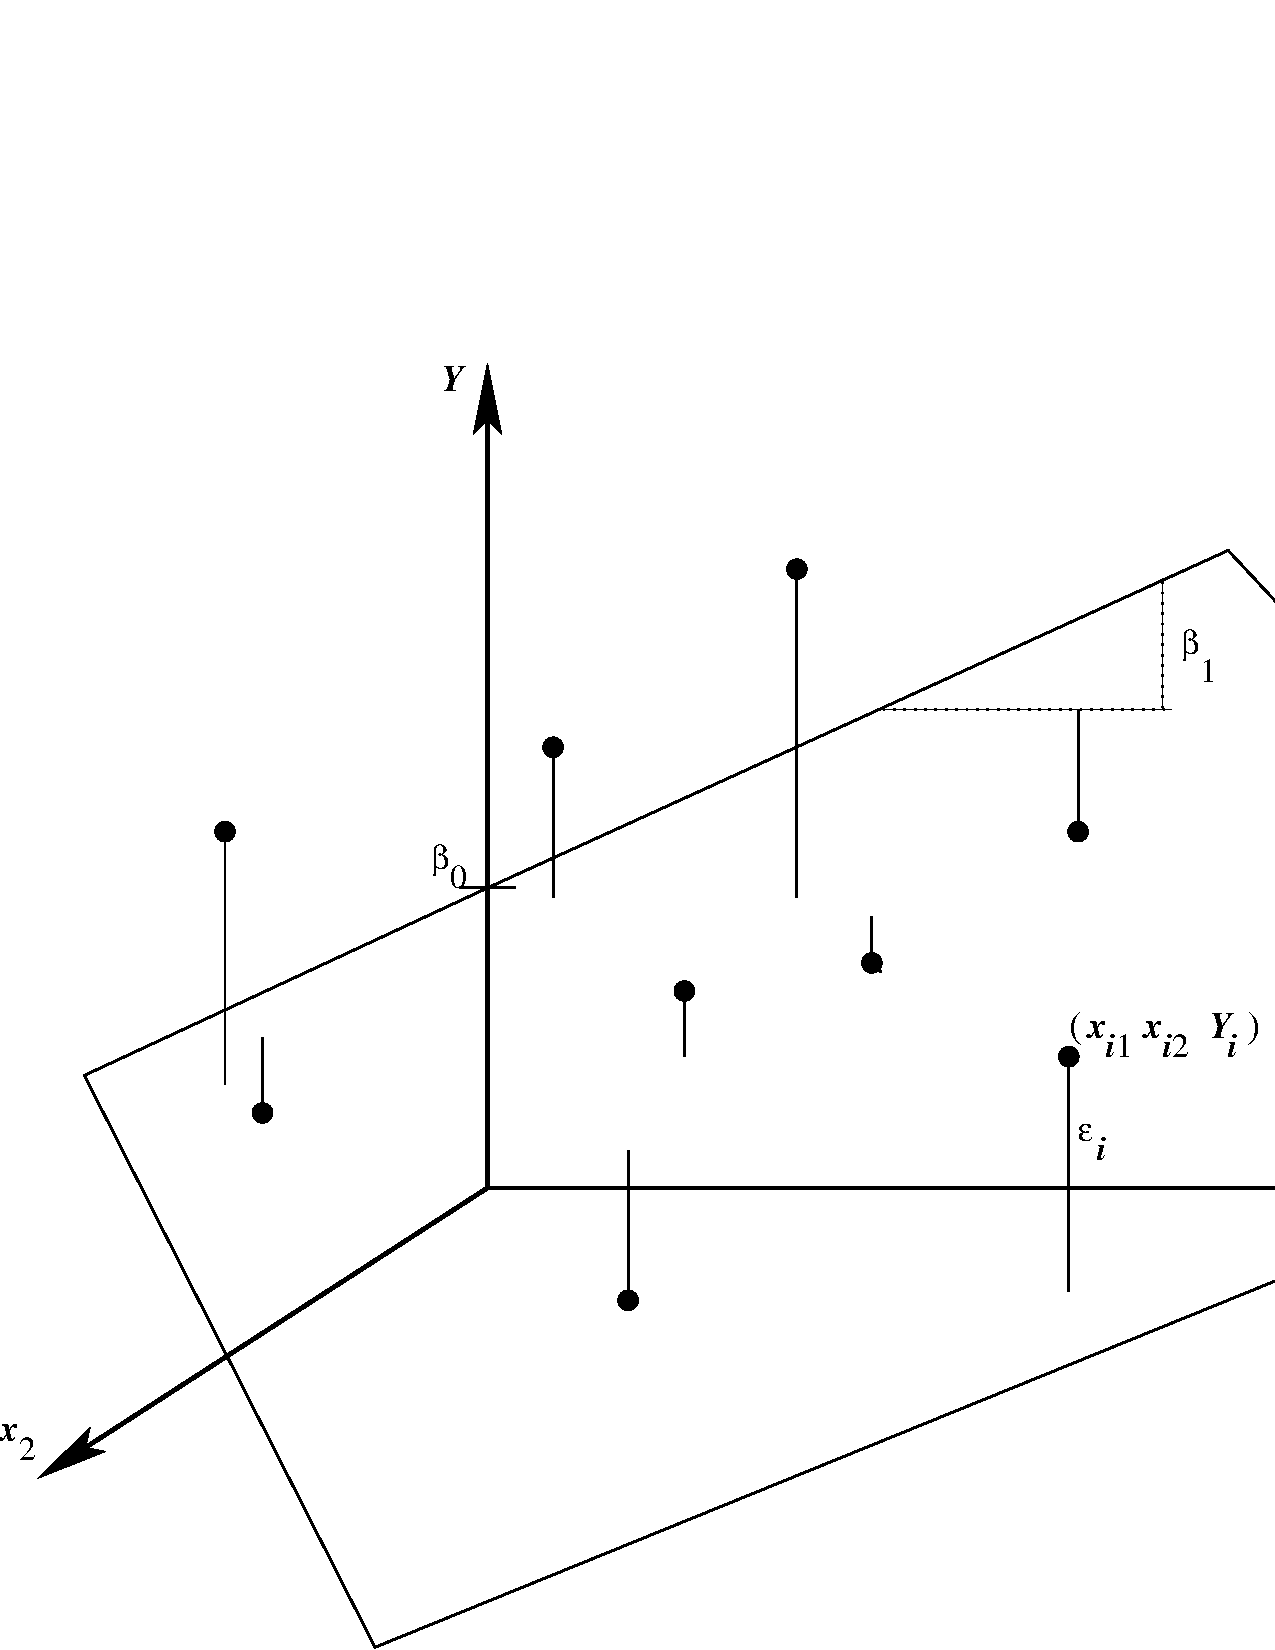
\includegraphics[scale=0.35, trim={0 0 0 5cm}]
{Chap5-AjusterRLM/Figures/reg_mult.pdf}}
\caption{Représentation géométrique du modèle de régression linéaire multiple.}\label{fig:rlm}
\end{figure}



\section{Estimation des coefficients}
\label{sec:EstimationParamètres}

Les coefficients de régression $\beta_0,\, \beta_1, \, \dots, \, \beta_p$ doivent être estimés. Nous présentons dans cette section la méthode des moindres carrés et une approche géométrique. Il est aussi possible d'utiliser la méthode du maximum de vraisemblance pour obtenir des estimateurs des coefficients, ce qui ne sera pas présenté dans le cadre de la RLM.

\subsection{Méthode des moindres carrés}
\label{sec:EstimationRLMMoindresCarrés}

Comme dans le cas de la régression linéaire simple, on adopte à nouveau le principe des moindres carrés de Legendre. On cherche par conséquent le vecteur $\bobeta$ qui minimise la somme des carrés des résidus ($\sum_{i=1} ^n{\widehat{\varepsilon}_i^2}$). Le vecteur des résidus s'exprime
	\[ \boeps = \left({\varepsilon}_1 , \, {\varepsilon}_2, \, ... , \, {\varepsilon}_n\right)^\top = \boY - \boX \bobeta, \]
on a alors
	\[\sum_{i=1}^n {\varepsilon}_i^2= \boeps^\top \boeps= (\boY - \boX \bobeta)^\top (\boY - \boX \bobeta)= f(\bobeta).\]
La fonction $f(\hbobeta)$ s'écrit comme
\begin{eqnarray*}
	f(\bobeta)
    &=& \left[\boY^\top - (\boX \bobeta)^\top\right](\boY - \boX \bobeta) \\
	&=& \boY^\top \boY - \boY^\top \boX \bobeta - (\boX\bobeta)^\top \boY + (\boX\bobeta)^\top (\boX\bobeta) \\
	&=& \boY^\top \boY - 2\bobeta^\top\boX^\top\boY  + \bobeta^\top\boX^\top  \boX\bobeta.
\end{eqnarray*}
Dans la dernière égalité on a que $\boY^\top\boX\bobeta=(\boX\bobeta)^\top\boY=\bobeta^\top\boX^\top\boY$ puisque ces trois quantités sont des scalaires.

Ainsi, pour minimiser $\sum_{i=1} ^n{\widehat{\varepsilon}_i^2}$, il faut dériver $f(\bobeta)$ par rapport à $\bobeta$, puis évaluer la dérivée au point $\hbobeta$ et égaler à 0. En utilisant les notions de la section \ref{sec:Deriver}, on obtient
\[\frac{\partial f(\bobeta)}{ \partial \bobeta} = -2\boX^\top \boY + 2\boX^\top \boX \bobeta.\]
On a ensuite 
\begin{align}
    -2\boX^\top \boY + 2\boX^\top \boX \hbobeta &= 0 \nonumber\\
    \boX^\top \boX \hbobeta  &= \boX^\top \boY \nonumber\\
    \hbobeta  &= \left( \boX^\top \boX \right)^{-1}\boX^\top \boY , \label{eq:est_beta}
\end{align}
si $\boX^\top \boX$ est inversible (de plein rang).
Notons que
\begin{eqnarray*}
	\underbrace{\hbobeta}_{p'\times 1}=\underbrace{(\boX^\top \boX)^{-1}}_{p'\times p'} \underbrace{\boX^\top}_{p'\times n} \underbrace{\boY}_{n\times 1}.
\end{eqnarray*}

\begin{remarque}
La matrice $\boX^\top \boX$ n'est pas  inversible si le nombre d'observations $n$ est inférieur au nombre de paramètres à estimer $p'$, ou si une ligne de cette matrice est une combinaison linéaire des autres. Dans le premier cas, une méthode d'estimation de modèle plus complexe peut être utilisée, comme présenté à la section \ref{sub:lasso}. Dans le second cas, une variable peut être retirée du modèle, voir le chapitre \ref{sec:Multicolinéarité} sur la multicolinéarité.
\end{remarque}

\begin{exemple}
    {\bf Application au cas $p=1$}

    Comme vu dans l'exemple \ref{RLSRLM1}, le modèle de RLS est un cas particulier du modèle de RLM. Vérifions que l'équation (\ref{eq:est_beta}) mène aux estimateurs obtenus au Chapitre \ref{sec:AjusterRLS}.
    En reprenant la notation de l'exemple \ref{RLSRLM1}, on a que 
    \begin{align*}
        \boX^\top \boX
        &=
        \begin{pmatrix}
        1 & 1 & \cdots & 1   \\
        x_1 & x_{2} & \cdots & x_n  
    \end{pmatrix}
        \begin{pmatrix}
        1 & x_{1}   \\
        1 & x_{2}  \\
        \vdots & \vdots \\
        1 & x_{n}  
    \end{pmatrix}
    = \begin{pmatrix}
        n & \sum\limits_{i=1}^n x_i  \\[4mm]
        \sum\limits_{i=1}^n x_i  & \sum\limits_{i=1}^n x_i^2
    \end{pmatrix}
    = 
    \begin{pmatrix}
        n & n \overline{x} \\[4mm]
         n \overline{x}   & \sum\limits_{i=1}^n x_i^2
    \end{pmatrix}
    \end{align*}
   On calcule l'inverse de cette matice $2\times 2$. Le déterminant est 
   $$	\mathrm{det}(\boX^\top\boX) = n \sum_{i=1}^n x_i^2 - n^2\overline{x}^2
	= n \left(\sum_{i=1}^n x_i^2 - \sum_{i=1}^n \overline{x}^2\right)
	= n \sum_{i=1}^n  (x_i^2 - \overline{x}^2)
	= n \sum_{i=1}^n  (x_i - \overline{x})^2
	= n S_{xx}. $$
    Alors
    \begin{align*}
        \left(\boX^\top \boX\right) ^{-1}
        =  \frac{1}{nS_{xx}} \begin{pmatrix}
            \sum\limits_{i=1}^n x_i^2 & -n\overline{x}\\
            -n\overline{x} & n 
        \end{pmatrix}.
    \end{align*}
    Calculons $\hbobeta$,
    \begin{align*}
        \hbobeta
        &= (\boX^\top \boX)^{-1} \boX^\top \boY \\
        &= \frac{1}{nS_{xx}} \begin{pmatrix}
            \sum\limits_{i=1}^n x_i^2 & -n\overline{x}\\
            -n\overline{x} & n 
            \end{pmatrix}
            \begin{pmatrix}
                1 & 1 & \cdots & 1   \\
                x_1 & x_{2} & \cdots & x_n  
            \end{pmatrix}
            \begin{pmatrix}
                Y_1 \\ \vdots \\ Y_n
            \end{pmatrix} \\
        &= \frac{1}{nS_{xx}} \begin{pmatrix}
            \sum\limits_{i=1}^n x_i^2 & -n\overline{x}\\
            -n\overline{x} & n 
            \end{pmatrix}
            \begin{pmatrix}
                \sum\limits_{i=1}^n Y_i \\[4mm]
                \sum\limits_{i=1}^n x_iY_i 
            \end{pmatrix} \\
        &= \frac{1}{nS_{xx}} \begin{pmatrix}
            n\overline{Y}\sum\limits_{i=1}^n x_i^2  - n\overline{x} \sum\limits_{i=1}^n x_i Y_i \\[4mm]
            -n\overline{x}\sum\limits_{i=1}^n Y_i  + n \sum\limits_{i=1}^n x_i Y_i
        \end{pmatrix} \\
        &= \begin{pmatrix}
        \frac{\displaystyle\overline Y\left( \sum\limits_{i=1}^n x_i^2-n\overline x^2\right)-\overline x\left(\sum\limits_{i=1}^n  x_i Y_i-n\overline x\overline Y\right)}{\displaystyle S_{xx}} \\
            \frac{\displaystyle  \sum\limits_{i=1}^n x_i Y_i - n\overline{x} \overline{Y}}{\displaystyle S_{xx}} 
        \end{pmatrix} \\
        &= \begin{pmatrix}
        \frac{\displaystyle \overline{Y}S_{xx} - \overline{x}S_{xy}}{\displaystyle S_{xx}} \\
            \frac{\displaystyle S_{xy}}{\displaystyle S_{xx}}
        \end{pmatrix} 
        = \begin{pmatrix}
        \overline{Y} - \overline{x} \widehat{\beta}_1 \\
            \frac{\displaystyle S_{xy}}{\displaystyle S_{xx}}
        \end{pmatrix}
        = \begin{pmatrix}
            \widehat{\beta}_0 \\\widehat{\beta}_1
        \end{pmatrix}.
    \end{align*}
    On obtient les mêmes résultats qu'en \eqref{eq:beta0} et \eqref{eq:beta1chapeau}.
\end{exemple}


\subsection{Argument géométrique}
\label{sec:ArgumentGéométrique}

Il est possible d'obtenir l'estimateur (\ref{eq:est_beta}) à partir d'une approche géométrique. Le vecteur $\boY$ peut s'écrire comme une combinaison linéaire des colonnes de $\boX$, plus une erreur $\boeps$:
\begin{align*}
\boY &= \boX \bobeta + \boeps \\
    &=   \begin{pmatrix}
        \bf 1 & \bold{x}_{1}  & \cdots & \bold x_{p}  
    \end{pmatrix}
    \begin{pmatrix}
        \beta_0 \\
        \vdots \\
        \beta_p 
    \end{pmatrix}
    +    \boeps \\
    &= \beta_0 {\bf 1} + \beta_1 {\bold x}_{1} + \dots + \beta_p \bold x_{p} + \boeps,
\end{align*}
avec $\bold 1 = (1, \dots, 1)^\top$ $\bold x_j = (x_{1j}, \dots, x_{nj})^\top$.

Soit le sous-espace vectoriel formé par les colonnes de $\boX$. Si $\boX$ est de plein rang (inversible), cet espace aura $p'=p+1$ dimensions. Pour estimer les paramètres du modèle de régression linéaire multiple, on peut projeter $\boY$ dans le sous-espace vectoriel engendré par les colonnes $\boX$. Cette projection orthogonale permet d'obtenir la partie de $\boY$ qui est linéairement expliquées par les colonnes de $\boX$.

Soit $\boH$ la matrice chapeau, c'est-à-dire la matrice de projection orthogonale dans l'espace engendré par les colonnes de $\boX$ (voir la section \ref{sec:MatriceChapeau} pour plus de détails sur cette matrice). 
Le vecteur $\hY$ est le vecteur de valeurs prédites et correspond à la projection orthogonale de $\boY$ sur le sous-espace engendré par les colonnes de $\boX$,
\begin{align*}
    \hY = \boH \boY.    
\end{align*}
Ainsi, $\hY$ s'exprime comme une combinaison linéaire des vecteurs $\bf 1$ et $\bold x_j$, $j=1, \dots, p$.
Le vecteur de résidus $\hboeps$ s'écrit 
$$\hboeps = \boY-\hY = (\boI_n-\boH)\boY.$$ 
Ainsi, le vecteur $\hboeps$ est perpendiculaire au sous-espace engendré par les colonnes de $\boX$, il est une projection de $\boY$ dans le sous-espace perpendiculaire à celui engendré par les colonnes de $\boX$. Toujours en considérant $\boX$ de plein rang, ce sous-espace est de dimension $(n-p')$. La projection orthogonale permet de minimiser la somme des résidus au carré, c'est-à-dire $\hboeps'\hboeps$. L'orthogonalité de $\hY$ et $\hboeps$ revient à dire que $\cov[\hboeps, \hY] = 0$. En effet, des vecteurs orthogonaux sont des vecteurs non corrélés. Dans le cas gaussien, ceci implique de plus que ces vecteurs sont indépendants.
La figure \ref{fig:geometrie} représente géométriquement le cas où $n=3$ $p'=2$. 


\definecolor{bleufonce}{RGB}{30,74,126}
\definecolor{bleuclair}{RGB}{64,120,190}
\definecolor{planbleu}{RGB}{231,239,248}

\begin{figure}
    \centering
    \begin{tikzpicture}[line cap=round,
                    line join=round,
                    >=stealth,
                    scale=1.15]
% Sommets du plan
\coordinate (A) at (0,0);
\coordinate (B) at (5.8,-0.75);
\coordinate (C) at (7.6,1.75);
\coordinate (D) at (1.8,2.5);
% Origine des vecteurs, projection et extrémité de Y
\coordinate (O) at (2.30,0.52);
\coordinate (P) at (4.72,1.02);
\coordinate (Y) at (4.72,3.92);
% Plan vectoriel
\filldraw[fill=planbleu,
        fill opacity=0.6,
        draw=bleufonce,
        line width=1.2pt] (A) -- (B) -- (C) -- (D) -- cycle;
% Vecteur Y
\draw[->, color=bleuclair, line width=1.1pt] (O) -- (Y);
% Projection de Y sur le plan
\draw[->, dotted, color=bleuclair, line width=1.1pt] (O) -- (P);
% Résidu orthogonal
\draw[->, dotted, color=bleuclair, line width=1.1pt] (P) -- (Y);
% Symbole d'angle droit
\coordinate (Q1) at ($(P)!0.18!(O)$);
\coordinate (Q2) at ($(P)!0.16!(Y)$);
\coordinate (Q3) at ($(Q1)+(Q2)-(P)$);
\draw[color=bleuclair, line width=0.9pt] (Q1) -- (Q3) -- (Q2);
% Étiquettes
\node[above left=1pt, font=\large] at ($(O)!0.68!(Y)$) {$\bf{Y}$};
\node[below=5pt, rotate=10, font=\large] at ($(O)!0.68!(P)$)
    {$\widehat{\boY}=\boH\boY$};
\node[right=8pt, font=\large] at ($(P)!0.60!(Y)$)
    {$\widehat{\boeps}=(\boI_n-\boH)\mathbf{Y}$};
\end{tikzpicture}
    \caption{Représentation géométrique de la régression dans le cas où $p=1$ et $n=3$.}
    \label{fig:geometrie}
\end{figure}


Pour obtenir $\hbobeta$ sous cette approche, on peut utiliser le fait que l'on veut écrire $\widehat{\boY} = \boX \hbobeta$ et que $\hY$ est perpendiculaire à $\hboeps$,
\begin{align*}
    \hY^\top \hboeps &= 0 \\
    \left(\boX \hbobeta\right)^\top \hboeps &= 0  \\
     \hbobeta^\top \boX^\top \hboeps &= 0,  \\
 \intertext{ainsi}    
    \boX^\top \hboeps &= 0  \\
    \boX^\top(\boY-\boX\hbobeta) &= 0 \\
    \boX^\top\boY - \boX^\top\boX\hbobeta &= 0 \\
    \boX^\top\boY &= \boX^\top\boX\hbobeta  \\
    \left(\boX^\top\boX\right)^{-1}\boX^\top\boY &= \hbobeta  
\end{align*}
et on retrouve les résultats obtenus avec les moindres carrés, soit l'équation (\ref{eq:est_beta}).






\section{Exemple}

Cet exemple est tiré de \citet[][Exemple 14.1]{Hin_Mon_Gol_Bor:12}.
%\citet{Rag_Ber:01} exposent une analyse consistant à trouver un modèle de prévision des meurtrissures des pommes durant le tri et l'emballage.
Des expériences en laboratoire ont montré que le diamètre des meurtrissures (en mm) peut être expliqué en fonction de la hauteur de chute (en mm) et de la masse volumique des fruits (en g/cm$^3$). Le Tableau \ref{exp_data} présente des données typiques de ce type d'expérience.

Le modèle de régression linéaire multiple s'exprime sous forme matricielle comme
$$
\underbrace{\left(
\begin{array}{c}
3,62  \\
7,27  \\
2,66 \\
1,53 \\
\vdots \\
5,23  \\
\end{array} \right)}_{20\times 1}
 =  \underbrace{\left(\begin{array}{ccc}
            1	&      303,7  & 0,9     \\
            1	&      366,7  & 1,04    \\
            1 &         336,8 & 1,01 \\
            1 &           304,5 & 0,95 \\
            \vdots & \vdots & \vdots   \\
            1	&      351,4  & 0,96
\end{array}\right)}_{20\times 3}
\underbrace{\left(\begin{array}{c}
\beta_0 \\
\beta_1 \\
\beta_2
\end{array} \right)}_{3\times 1}+
\underbrace{\left(\begin{array}{c}
\varepsilon_1 \\
\varepsilon_2 \\
\varepsilon_3 \\
\varepsilon_4 \\
\vdots \\
\varepsilon_{20}
 \end{array}
 \right)}_{20\times 1}
 $$
Selon l'équation (\ref{eq:est_beta}), on sait que $\hbobeta=(\boX^\top\boX)^{-1}\boX^\top \boY$.
La matrice $\boX^\top\boX$ est
\begin{eqnarray*}
\boX^\top\boX & = & \left(
\begin{array}{cccc}
1 & 1 & \cdots & 1 \\
303,7 & 366,7 & \cdots & 351,4 \\
0,90 & 1,04 & \cdots & 0,96
\end{array}
\right)
\left(
\begin{array}{ccc}
1 & 303,7 & 0,90 \\
1 & 366,7 & 1,04 \\
\vdots & \vdots & \vdots \\
1 & 351,4 & 0,96
\end{array}
\right) \\
& = & \left(
\begin{array}{ccc}
20 & 7767,8 & 19,33 \\
7767,8 & 3201646 & 7791,878 \\
19,93 & 7791,878 & 19,9077
\end{array}
\right).
\end{eqnarray*}
Le vecteur $\boX^\top\boY$ s'exprime comme
\begin{eqnarray*}
\left(
\begin{array}{cccc}
1 & 1 & \cdots & 1 \\
303,7 & 366,7 & \cdots & 351,4 \\
0,90 & 1,04 & \cdots & 0,96
\end{array}
\right)
\left(
\begin{array}{c}
3,62 \\
7,27 \\
\vdots \\
5,23
\end{array}
\right)
=
\left(
\begin{array}{r}
120,79 \\
51129,17 \\
122,70
\end{array}
\right).
\end{eqnarray*}
On en déduit donc que
\begin{eqnarray*}
\left(
\begin{array}{c}
\hat\beta_0 \\
\hat\beta_1 \\
\hat\beta_2
\end{array}
\right)
& = &
\left(
\begin{array}{ccc}
20 & 7767,8 & 19,33 \\
7767,8 & 3201646 & 7791,878 \\
19,93 & 7791,878 & 19,9077
\end{array}
\right)^{-1}
\left(
\begin{array}{r}
120,79 \\
51129,17 \\
122,70
\end{array}
\right) \\
& = &
\left(
\begin{array}{rrr}
24,63666 & 0,005321 & -26,74679 \\
0,005321 & 0,0000077 & -0,008353 \\
-26,74679 & -0,008353 & 30,096389
\end{array}
\right)
\left(
\begin{array}{r}
120,79 \\
51129,17 \\
122,70
\end{array}
\right) \\
& = &
\left(
\begin{array}{r}
-33,8310 \\
0,0134 \\
34,8900
\end{array}
\right).
\end{eqnarray*}
Par conséquent, le modèle de régression ajusté s'écrit 
$$\hat Y=-33,831+0,0134x_1+34,890x_2.$$
L'espérance du diamètre moyen des meurtrissures d'une pêche de masse volumique nulle lancée d'une hauteur nulle (très hypothétique comme valeur!) est de $-33,831$ mm. L'augmentation d'un mm de la hauteur de la chute est associée à une augmentation attendue de 0,0134 mm du diamètre moyen des meurtrissures, pour une masse volumique constante. De même, l'augmentation d'un $g/cm^3$ de la masse volumique d'une pêche est associée à une augmentation attendue de $34,890$ mm du diamètre moyen des meurtrissures, pour une hauteur de chute constante.


\begin{table}[htb!]
\caption{Données pour l'exemple des meurtrissures de pêches}
\label{exp_data}
\begin{tabular}{|c|c|c|c|} \hline
numéro &  diamètre des meurtrissures  & hauteur de chute  & masse volumique  \\
 & [mm] & [mm] & [g/cm$^3$] \\
        & $Y_i$        & $x_{i1}$      &  $x_{i2}$ \\ \hline
 1   &   3,62  &   303,7  & 0,90      \\
 2   &   7,27  &   366,7  & 1,04     \\
 3   &   2,66  &  336,8   & 1,01     \\
 4   &   1,53  &  304,5   & 0,95      \\
 5   &   4,91  &  346,8   & 0,98      \\
 6   &   10,36 &   600,0    & 1,04       \\
 7   &   5,26  &   369,0    & 0,96       \\
 8   &   6,09  &   418,0    & 1,00           \\
 9   &   6,57  &   269,0    & 1,01        \\
 10  &   4,24  &   323,0    & 0,94         \\
 11  &   8,04  &   562,2  & 1,01          \\
 12  &   3,46  &   284,2  & 0,97           \\
 13  &   8,50   &   558,6  & 1,03           \\
 14  &   9,34  &   415,0    & 1,01            \\
 15  &   5,55  &   349,5  & 1,04            \\
 16  &   8,11  &   462,8  & 1,02            \\
 17  &   7,32  &   333,1  & 1,05            \\
 18  &   12,58 &   502,1  & 1,10            \\
 19  &   0,15  &   311,4  & 0,91            \\
 20  &   5,23  &   351,4  & 0,96            \\   \hline
\end{tabular}

\end{table}

